\chapter{Neural Networks}
\label{chapter:neural networks}

Applicability of models that comprised linear combinations of \textbf{fixed basis functions} is limited by the curse of dimensionality.In order the apply such models to large-scale problems,it is necessary to adapt the basis functions to the data.

Support vector machines and relevance vector machine \textbf{choose a subset from a fixed set of basis functions} and results in much sparser models.

An alternative approach is to fix the number of basis functions in advance but allow them to be \textbf{adaptive},in other words to use parametric forms for the basis function 
\section{Feed-forward Network Functions}
The linear models are based on linear combinations of fixed nonlinear basis functions $\phi_j(\vec{x})$ and take the form
\begin{align}
    y(\vec{x},\vec{w}) = f(\sum_{j=1}^{M}w_j\phi_j(\vec{x})) = f(\vec{w}^T\vec{\phi}(\vec{x}))
\end{align}
where $f(\cdot)$ is a nonlinear activation function in the case of classification and is the identity in the case of regression.

Neural network model can be described a series of functional transformations.First construct $M$ linear combinations of the input variables $x_1,\ldots,x_D$ in the form
\begin{align}
    a_j^{(l+1)} &= \sum_{i=1}^{D}w_{ji}^{(l)}x_i+w_{j0}^{(l)} \\
	    &= \vec{w}^{(l)}\vec{x}^{(l)}
\end{align}
where $j=1,\ldots,M$,and the superscript $(l)$ indicates the $l-the$ layer of the network.We refer the parameters $w_{ji}^{(l)}$ as \textbf{weights} and $w_{j0}^{(l)}$ as \textbf{biases}.The quantity $a_j$ are known as \textbf{activations}.Each of them is then transformed using \textbf{activation function} $h(\cdot)$ to give
\begin{align}
    z_j=h(a_j)
\end{align}
These quantities correspond to the outputs of the basis functions in linear model that,in the context of neural networks,are called \textbf{hidden units}.The nonlinear functions $h(\cdot)$ are generally chosen to be sigmoidal or the '$tanh$' function.

The transformation of the following layer of the network,combine these values to give \textbf{output unit activations}
\begin{align}
    a_k=\sum_{j=1}^{M}w_{kj}^{(2)}z_j+w_{k0}^{(2)}
\end{align}
where $k=1,\ldots,K$,and $K$ is the total number of outputs.

\begin{figure}
    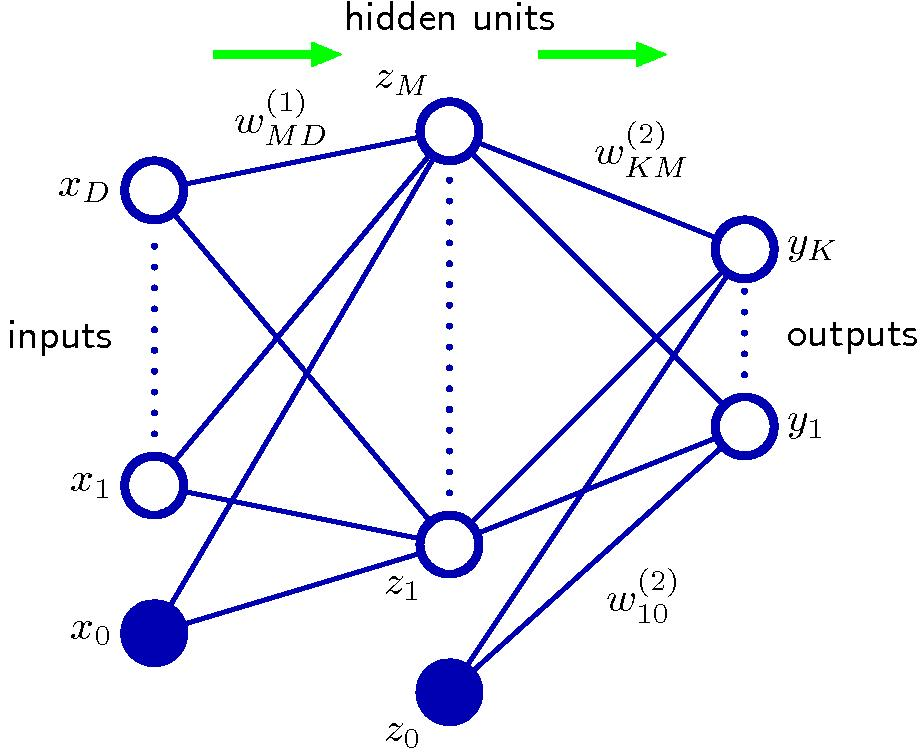
\includegraphics[ ]{figures/prml/Figure5.1.jpg}
    \caption{Network diagram for two-layer neural network}
\end{figure}

For regression,$y_k=a_k$ and binary classification,we can use $y_k=\sigma(a_k)=\dfrac{1}{1+\exp(-a)}$.Finally,for multiclass problems,a \textbf{softmax} activation function is used.\textbf{Unit activation function} is discussed later.

The process of evaluating the output of the network diagram is interpreted as a \textbf{forward propagation} of information through the network.Deterministic rather than stochastic variables of internal nodes do not represent probabilistic graphical models.Each (hidden or output) unit in such network computes a function given by
\begin{align}
    z_k=h(\sum_j w_{kj}z_j)
\end{align}
where the sum runs over all units that send connections to unit $k$ (including the bias parameter).

\subsection{Weight-space symmetries}
Consider a two-layer network as shown before.For $M$ hidden units,there will be $M$ 'sign-flip' symmetries,i.e.,$2^M$ equivalent weight vectors.Similarly,interchanging the values of all the weights(and the bias) can give rise to the same mapping function from inputs to outputs represented by the network.There will be $M!$ equivalent weight vectors.The network have an overall weight-space symmetry factor of $M!2^M$.


\section{Network Training}
Given a training set comprising a set of input vectors ${\vec{x}_n}$,where $n=1,\ldots,N$,together with a corresponding set of target vectors ${\vec{t}_n}$,we minimize the error function.We can provide a probabilistic interpretation to the network outputs.

For regression,and for the moment we consider a single target variable $t$ that can take any real value.We assume that $t$ has a Gaussian distribution with an $\vec{x}$-dependent mean,which is given by the output of the neural network,so that
\begin{align}
    p(t|\vec{w},\vec{w})=\mathcal{N}(t|y(\vec{x},\vec{w}),\beta^{-1})
\end{align}
where $\beta$ is the precision (inverse variance) of the Gaussian noise.Maximize the likelihood function as in linear models.View the network as having an output activation function that id the identity,so that $y_k=a_k$.The corresponding sum-of-squares error function has the property
\begin{align}\label{eqn:output activation function derivative}
    \dfrac{\partial E}{\partial a_k}=\dfrac{\partial E}{\partial y_k}=y_k - t_k
\end{align}

For binary classification in which $t\in{0,1}$,consider a network having a single output whose activation function is a logistic sigmoid
\begin{align}
    y=\sigma(a)=\dfrac{1}{1+\exp(-a)}
\end{align}
We can interpret $y(\vec{x},\vec{w})$ as the conditional probability $p(\mathcal{C}_1|\vec{x})$.the conditional distribution of targets given inputs is then a Bernoulli distribution of the form
\begin{align}
    p(t|\vec{x},\vec{w})=y(\vec{x},\vec{w})^t\{{1-y(\vec{x},\vec{w})}^{1-t}\}
\end{align}

For $K$ separate binary classifications,the conditional distribution of the targets is
\begin{align}
    p(\vec{t}|\vec{x},\vec{w})=\prod_{k=1}^{K}y_k(\vec{x},\vec{w})^t_k[1-y(\vec{x},\vec{w})]^{1-t_k}
\end{align}
Taking the negative logarithm of the corresponding likelihood function,we get \textbf{cross-entropy} error function
\begin{align}
    E(\vec{w})=-\sum_{n=1}^{N}\sum_{k=1}^{K}{t_{nk}\ln y_{nk}+(1-t_{nk})\ln(1-y_{nk})}
\end{align}
The derivative of the error function with respect to the \textbf{activation} for a particular output unit is
\begin{align}
    \dfrac{\partial E_n}{\partial a_k}
    &=\dfrac{\partial {-\sum_{k=1}^{K}{t_{nk}\ln y_{nk}+(1-t_{nk})\ln(1-y_{nk})} }}{\partial a_k} \\
    &=-{t_{k} \dfrac{y_{k}(1-y_{k})}{y_{k}} +(1-t_{k}\dfrac{-y_{k}(1-y_{k})}{1-y_{k}}) } \\
    &={y_{k}-t_{k}}
\end{align}

Following the logistic regression,the \textbf{output unit activation} is given by the \textbf{softmax} function
\begin{align}
    y_k(\vec{x},\vec{w})=\dfrac{\exp(a_k(\vec{x},\vec{w}))}{\sum_j\exp(a_j(\vec{x},\vec{w})) }
\end{align}

\subsection{Parameter optimization}
Turn next to the task of finding a weight vector $\vec{w}$ which minimizes the chosen function $E(\vec{w})$.
\begin{figure}
    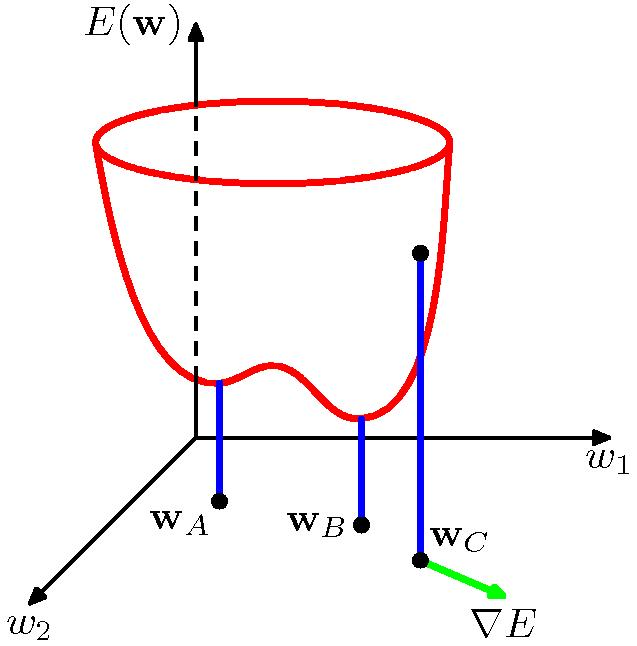
\includegraphics{figures/prml/Figure5.5.jpg}
    \caption{geometrical view of the error function $E(\vec{w})$ as a surface sitting over weight space.A is a local minimum and B is the global minimum.The local gradient of the error surface is given by the vector $\nabla E$.}
\end{figure}
Resort to \textbf{iterative} numerical procedures.Most techniques involve choosing some initial value $\vec{w}^{(0)}$ for weight vector and then moving through weight space in a succession of steps of the form
\begin{align}
    \vec{w}^{(\eta+1)}=\vec{w}^{(\eta)}+\Delta \vec{w}^{(\eta)}
\end{align}

Many algorithms make use of gradient information,evaluating $\nabla E(\vec{w})$  at the new weight vector $\vec{w}^{(\eta+1)}$.

\subsection{Local quadratic approximation}
Consider the \textbf{Taylor expansion} of $E(\vec{w})$ around some point in weight space.

\subsection{Use of gradient information}
It is possible to evaluate the gradient of an error function efficiently by means of the backpropagation procedure.Because each evaluation of $\nabla E$ brings $W$ items of information,we might hope to find the minimum of the function in $O(W)$ gradient evaluations.Each such evaluation takes only $O(W)$ steps and so the minimum can be now found in $O(W^2)$ steps.
\subsection{Gradient descent optimization}
\textbf{Batch gradient descent}
\begin{align}
    \vec{w}^{(\tau+1)}=\vec{w}^{(\tau)}-\eta\nabla E(\vec{w})^{(\tau)}
\end{align}
where the parameter $\eta>0$ is known as the \textbf{learning rate}.

More efficient methods than this poor algorithm are \textbf{conjugate gradients} and \textbf{quasi-Newton} methods,which are more robust and much faster.\textbf{On-line} version of gradient has also proved useful in practice.On-line gradient descent,known as \textbf{sequential gradient descent } or \textbf{stochastic gradient descent},makes an update to the weight vector based on one data point at a time,so that
\begin{align}
    \vec{w}^{(\tau+1)}=\vec{w}^{(\tau)}-\eta \nabla E(\vec{w}^{(\tau)})
\end{align}


\section{Error Backpropagation}
The goal in this section is to find an efficient technique for evaluating the gradient of an error function $E(\vec{w})$ for a feed-forward neural network.This can be achieved using a local message passing scheme in which information is sent alternately forwards and backwards through the network,known as \textbf{error backpropagation} or \textbf{backprop}.

\subsection{Evaluation of error-function derivatives}
Many error functions of practical interest,for instance those defined by maximum likelihood for a set of i.i.d data,comprise a sum of terms,on for each data point,so that
\begin{align}
    E(\vec{w})=\sum_{n=1}^{N}E_n(\vec{w})
\end{align}

In a general feed-forward network,each unit computes a weighted sum of its inputs of the form
\begin{align}
    a_j=\sum_i w_{ji} z_i
\end{align}
where $z_i$ is the activation of a unit that sends a connection to unit $j$ and $w_{ji}$ is the weight associated with that connection.The sum is transformed by an activation function $h(\cdot)$ to give the activation $z_j$ of unit $j$ in the form
\begin{align}
    z_j=h(a_j)
\end{align}

Evaluate the derivate of $E_n$ with respect to a weight $w_{ji}$,applying the \textbf{chain rule} for partial derivatives
\begin{align}
    \dfrac{\partial E_n}{\partial w_{ji}}=\dfrac{\partial E_n}{\partial \vec{a}_j}\dfrac{a_j}{\partial w_{ji}}
\end{align}
Now introduce a notation
\begin{align}
    \delta_j \equiv \dfrac{\partial E_n}{\partial a_j}
\end{align}
referred as \textbf{errors}.
Using the sum form
\begin{align}
    \dfrac{\partial a_j}{\partial w_{ji}} = z_i
\end{align}
Substituting them back
\begin{align}
    \dfrac{\partial E_n}{\partial w_{ji}}=\delta_j z_i.
\end{align}
For the output units,we have
\begin{align}
    \delta_k=y_k-t_k
\end{align}

For hidden units,make use of the chain rule for partial derivatives
\begin{align}
    \delta_j\equiv \dfrac{\partial E_n}{\partial a_j}=
    \sum_k \dfrac{\partial E_n}{\partial a_k}\dfrac{\partial a_k}{\partial a_j} \\
\end{align}
where the sum runs over all units $k$ to which unit $j$ sends connections.
\begin{align}
    \because \delta_k &= \dfrac{\partial E_n}{\partial a_k}\\
    \therefore
    \delta_j\equiv \dfrac{\partial E_n}{\partial a_j} &=
    \sum_k \dfrac{\partial E_n}{\partial a_k}\dfrac{\partial a_k}{\partial a_j} \\
    &=\sum_k \delta_k\dfrac{\partial a_k}{\partial a_j} \\
    &=\sum_k \delta_k h'(a_j)w_{kj} \\
    &= h'(a_j)\sum_k w_{kj}\delta_k
\end{align}

\subsubsection{back-propagation algorithm wrap-up}

We'll use $\vec{w}_{ij}^{l}$ to denote the \textbf{weight} for the connection from the $k$th neuron in the $(l-1)$th layer to the $j$th neuron in the $(l)$th layer.And $b_j^l$  for the bias of the $j$th neuron in the $l$th layer, $a_j^l$ for the activation(weighted input) of the $j$th neuron in the $l$th layer,$\sigma$ denotes the element-wise activation function,$z_j^l$ denotes the output of $j$th neuron in the $l$th layer.
Then we have
\begin{align}
	\vec{a}^l &\equiv \vec{W}^l \vec{z}^{l-1}+\vec{b}^l \\
	\vec{z}^{l} &\equiv \sigma(\vec{a}^{l})
\end{align}

$s\odot t$ denotes \textbf{element-wise product} of two matrices (vectors):
\begin{align}
(s\odot t)_j = s_jt_j
\end{align}

Define the error $\sigma_j^l$ of neuron $J$ in the layer $l$ by
\begin{align}
\vec{\delta}^l_j \equiv \frac{\partial C}{\partial \vec{a}^l_j}
\end{align}

Using \textbf{chain rule of derivatives},the error in the output layer is:
\begin{eqnarray} 
\delta^L_j &=& \frac{\partial C}{\partial a^L_j} \\
&=& \sum_k \frac{\partial C}{\partial z^L_k} \frac{\partial z^L_k}{\partial a^L_j} \\
&=& \frac{\partial C}{\partial z^L_j} \frac{\partial z^L_j}{\partial a^L_j},\text{if output only depends on same neuron's input } \\
&=& \frac{\partial C}{\partial \vec{z}^L_j} \sigma'(\vec{a}^L_j).
\end{eqnarray}
And the matrix-based form is:
\begin{eqnarray} 
\delta^L & = & \nabla_z C \odot \sigma'(a^L). \\
\delta^L & = &\Sigma'(a^L) \nabla_z C,
\end{eqnarray}
where $\Sigma'(z^L)$ is a square matrix whose diagonal entries are the values $\sigma'(z^L)$, and whose off-diagonal entries are zero.

Propagation (recursive relationship) in hidden layer:
\begin{eqnarray} 
\delta_j^l &=& \frac{\partial C}{\partial a^l_j}\\
&=& \sum_k \frac{\partial C}{\partial a^{l+1}_k} \frac{\partial a^{l+1}_k}{\partial a^l_j}\\ 
&=& \sum_k \frac{\partial a^{l+1}_k}{\partial a^l_j} \delta^{l+1}_k, \\
\because a^{l+1}_k &=& \sum_j w^{l+1}_{kj} z^l_j +b^{l+1}_k = \sum_j w^{l+1}_{kj} \sigma(a^l_j) +b^{l+1}_k. \\
\therefore \frac{\partial a^{l+1}_k}{\partial a^l_j} &=& w^{l+1}_{kj} \sigma'(a^l_j) \\
\therefore
\delta^l_j &=& \sum_k w^{l+1}_{kj}  \delta^{l+1}_k \sigma'(a^l_j) \\
\delta^l &=& ((\vec{W}^{l+1})^T \delta^{l+1}) \odot \sigma'(\vec{a}^l), \\
\delta^l &=& \Sigma'(a^l) (w^{l+1})^T \delta^{l+1}.\\
\end{eqnarray}

Rate of change of cost with respect to bias in the network:
\begin{eqnarray}  
\frac{\partial C}{\partial b^l_j} 
&=\frac{\partial C}{\partial \vec{a}^l_j}\frac{\partial \vec{a}^l_j}{\partial b^l_j} \\
&= \frac{\partial C}{\partial \vec{a}^l_j} \cdot 1 
&=\vec{\delta}^l_j 
\end{eqnarray}

Rate of change of the cost with respect to any weight matrix in the network:
\begin{align}
    \frac{\partial C}{\partial w^l_{jk}} 
&= \frac{\partial C}{\partial \vec{a}^l_j}\frac{\partial \vec{a}^l_j}{\partial w^l_{jk}}\\
&= z^{l-1}_k \delta^l_j \\
\frac{\partial C}{\partial w} &= \vec{\delta_{\rm out}} \vec{z_{\rm in}}^T,
\end{align}

When dealing with \textbf{batch} training instances, we sum derivatives with respect to parameters over these instances.

\subsection{Efficiency of back propagation}

\subsection{The Jacobian matrix}
Back-propagation can also be applied to the calculation of other derivatives.Consider the evaluation of the \textbf{Jacobian matrix},whose elements are given by the derivatives of the network outputs with respects to the inputs
\begin{align}
    J_{ki}=\dfrac{\partial y_k}{\partial x_i}
\end{align}


\section{The Hessian Matrix}

\section{Regularization in Neural Networks}










\section{Mixture Density Networks}

\section{Bayesian Neural Networks}
